130. \begin{figure}[ht!]
\center{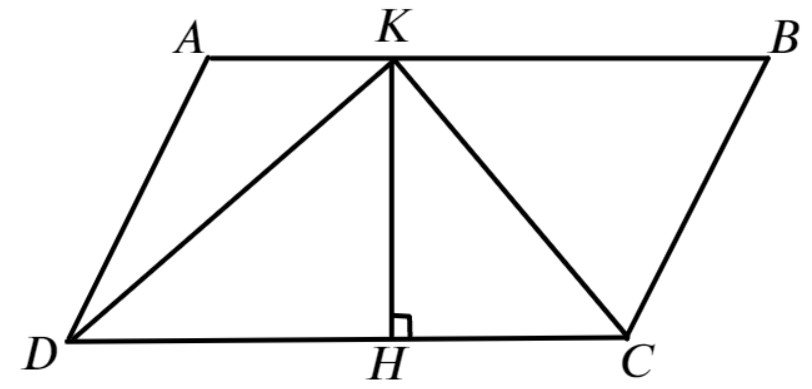
\includegraphics[scale=0.35]{g8-129.png}}
\end{figure}\\
Опусти высоту $LH$ из точки $L,$ она равна также и высоте параллелограмма. Тогда $S_{\Delta ALD}=\cfrac{1}{2}\cdot LH\cdot AD,\ S_{ABCD}=LH\cdot AD\Rightarrow
S_{ABCD}=2S_{\Delta ALD}=46.$\newpage\noindent
